\documentclass[a4paper,12pt]{article}
\usepackage[utf8]{inputenc}
% for comment blocks
\usepackage{verbatim}

% Larger borders -- we do not want do waste paper, even if it is only paper on screen =)
\usepackage[top=2.5cm, bottom=2.5cm, left=2cm, right=2cm]{geometry}

% No paragraph indentation
\setlength{\parindent}{0cm}

% Palatino font (nicer serif font: Times is for oldies)
\renewcommand*\rmdefault{ppl}

% Nested itemize list bullet style
\renewcommand{\labelitemi}{$\bullet$}
\renewcommand{\labelitemii}{$\circ$}
\renewcommand{\labelitemiii}{--}

% Math packages
\usepackage{amsmath}
\usepackage{amsfonts}
\usepackage{amssymb}

% Graphic packages
\usepackage{graphicx}
\usepackage{float}
\usepackage{adjustbox}
\usepackage{tikz}
\usepackage{forest,array}
\usetikzlibrary{shadows}

% Timing diagrams
\usepackage{tikz-timing}
\usetikztiminglibrary{arrows}

% Block diagrams
\usetikzlibrary{shapes}

% Graphs styles
\forestset{
  giombatree/.style={
    for tree={
      grow = east,
      parent anchor=east,
      child anchor=west,
      edge={rounded corners=2mm},
      fill=violet!5,
      drop shadow,
      l sep=10mm,
      edge path={
        \noexpand\path [draw, \forestoption{edge}] (!u.parent anchor) -- +(5mm,0) -- (.child anchor)\forestoption{edge label};
      }
    }
  }
}
\forestset{
  qtree/.style={
    for tree={
      parent anchor=south,
      child anchor=north,
      align=center,
      edge={rounded corners=2mm},
      fill=violet!5,
      drop shadow,
      l sep=10mm,
    }
  }
}

% Hides ugly links from the index
\usepackage[hidelinks]{hyperref}

% Landscape format pdf pagess
\usepackage{pdflscape}

% Overline in text mode
\makeatletter
\newcommand*{\textoverline}[1]{$\overline{\hbox{#1}}\m@th$}
\makeatother

% C highlight
\usepackage{listings}
\definecolor{customGreen}{RGB}{104,180,104}
\definecolor{customBlue}{RGB}{49,49,255}
\definecolor{customRed}{RGB}{150,0,0}
\lstdefinestyle{castyle} {
  language=C,
  breaklines = true,
  showstringspaces = false,
  basicstyle = \ttfamily,
  tabsize = 2,
	keywordstyle=\color{customBlue},
	identifierstyle=\color{black},
	commentstyle=\color{customGreen},
}
\lstset {
	basicstyle=\footnotesize\ttfamily,
	numbers=none,
	numbersep=5pt,
	stepnumber=1,
	firstnumber=1,
	tabsize=2,
	numberfirstline=true,
	basicstyle=\footnotesize\ttfamily,
	mathescape,
	extendedchars=true,
	breaklines=true,
	captionpos=b,
	postbreak=\raisebox{0ex}[0ex][0ex]{\ensuremath{\color{red}\hookrightarrow\space}},
	literate= % every possible kind of accent
	{à}{{\`a}}1
	{á}{{\'a}}1
	{í}{{\'i}}1
	{é}{{\'e}}1
	{è}{{\`e}}1
	{ý}{{\'y}}1
	{ì}{{\`i}}1
	{ú}{{\'u}}1
	{ù}{{\`u}}1
	{ó}{{\'o}}1
	{ò}{{\`o}}1
	{ě}{{\v{e}}}1
	{š}{{\v{s}}}1
	{č}{{\v{c}}}1
	{ř}{{\v{r}}}1
	{ž}{{\v{z}}}1
	{ď}{{\v{d}}}1
	{ť}{{\v{t}}}1
	{ň}{{\v{n}}}1
	{ů}{{\r{u}}}1
	{Á}{{\'A}}1
	{Í}{{\'I}}1
	{É}{{\'E}}1
	{Ý}{{\'Y}}1
	{Ú}{{\'U}}1
	{Ó}{{\'O}}1
	{Ě}{{\v{E}}}1
	{Š}{{\v{S}}}1
	{Č}{{\v{C}}}1
	{Ř}{{\v{R}}}1
	{Ž}{{\v{Z}}}1
	{Ď}{{\v{D}}}1
	{Ť}{{\v{T}}}1
	{Ň}{{\v{N}}}1
	{Ů}{{\r{U}}}1
	{°}{\textdegree}1
}

%%%%%%%%%%%%%%%%%%%%%%%%%%%%%%%%%%%%%%%%%%%%%%%%%%%%%%%%%%%%%%%%%%%%%%%%
% Specific commands for this document
\newcommand{\computername}{CA~19.32}
\newcommand{\memoryname}{Elephant}

% Monospace math environment
\everymath{\mathtt{\xdef\tmp{\fam\the\fam\relax}\aftergroup\tmp}} % inline math
\everydisplay{\mathtt{\xdef\tmp{\fam\the\fam\relax}\aftergroup\tmp}} % display math

% Title
\title{\memoryname{} DRAM}

% Authors
\author{G. Alvaro, F. Barbarulo, D. Comola, F. Fornaini, R. Polini, G.B. Rolandi}

\begin{document}
\maketitle
\tableofcontents

\clearpage
\clearpage

\section{Introduction}

This document describes the working details of the main memory and the main bus of the Computer~Architecture course computer.

\subsection{Bus}
Main bus is 16~bit wide address and 32~bit wide data bus.
Bus runs at 32~kHz.

\subsection{\memoryname{}}
\memoryname{} is a SDR DRAM, single data rate dynamic random access memory.

It can hold a total amount of 512~Kbit (64~KiB) of data, and can be accessed as 16~K locations of 32~bit (4 B) each.

\section{Main computer bus}
Physical main bus of \computername{} presents the following wires.

\begin{figure}[H]
\centering
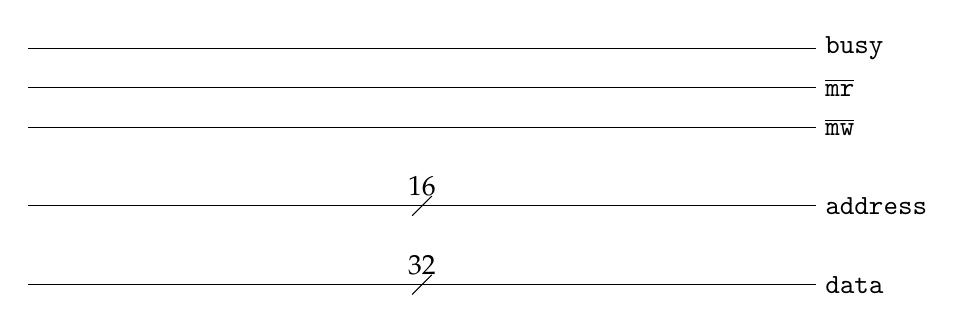
\begin{tikzpicture}
  % data wires
  \draw (0, 1)--(10, 1);
  \node at (5, 1){};
  \node [draw, strike out] at (5, 1){};
  \node [above] at (5, 1){32};
  \node [right] at (10, 1){\texttt{data}};

  % address wires
  \draw (0, 2)--(10, 2);
  \node at (5, 2){};
  \node [draw, strike out] at (5, 2){};
  \node [above] at (5, 2){16};
  \node [right] at (10, 2){\texttt{address}};

  % mw
  \draw (0, 3)--(10, 3);
  \node [right] at (10, 3){\textoverline{\texttt{mw}}};
  % mr
  \draw (0, 3.5)--(10, 3.5);
  \node [right] at (10, 3.5){\textoverline{\texttt{mr}}};

  % busy wire
  \draw (0, 4)--(10, 4);
  \node [right] at (10, 4){\texttt{busy}};
\end{tikzpicture}
\caption{main bus of \computername{}}
\end{figure}

% explanation
\begin{itemize}
  \item \textbf{busy:} this wire represents the busy status of the bus; the busy wire is active high.
  \item \textbf{\textoverline{mr}:} this wire issues a read data command, and instructs a module to put data from its internal structures onto the bus; the \textoverline{mr} wire is active low;
  \item \textbf{\textoverline{mw}:} this wire issues a write data command, and instructs a module to retrieve data from the bus and put into its internal structures; the \textoverline{mw} wire is active low;
  \item \textbf{address:} is 16~wires wide and selects the address from which/to which data must be read/written;
  \item \textbf{data:} is 32~wires wide and holds the actual data that must be read or written;
\end{itemize}

Thus, main computer bus can be represented in the simulation software by means of the structure described in \figurename~\ref{src:bus-h}:

\begin{figure}
\lstinputlisting[style=castyle]{../src/bus/bus.h}
\caption{Bus structure declaration}
\label{src:bus-h}
\end{figure}

Please note that the address line is 16~bit wide, but only 14 of them are actually used, since \memoryname{} holds only $2^{14} = 16K$ memory locations.
In particular, the 2 least significant bits are always assumed to be 0.

This choice has been agreed with the cache controller designers.

% BHA Protocol
\subsection{Bus handshake protocol}
In the simulation software, modules can:
\begin{itemize}
  \item be idle: this corresponds to the high impedance physical state;
  \item perform a read action from the bus;
  \item perform a write action on the bus;
\end{itemize}

Actions on bus must be performed in the simulation using the following protocol.

\begin{itemize}
  \item being idle: \texttt{set()} and \texttt{get()} methods of \texttt{Bus} class must not be called;
  \item read data: data can be read only upon receiving a message from another module. Data can be read using the \texttt{get()} method. It is not possible to read data more than once.
  \item write data: data can be written using the \texttt{set()} method;
  \begin{itemize}
    \item if busy bit is~1, data is not actually written onto the bus, \texttt{set()} method returns \texttt{false} and module must wait and schedule data writes onto the bus at a later time (eg. next clock tick);
    \item if busy bit is~0, data is actually written onto the bus and \texttt{set()} method returns \texttt{true}.
    Once written data to bus, destination module must be notified of the bus change by sending it a message using methods provided by the orchestrator.\\
    For the sake of simplicity, messages passed through the orchestrator can be tought as a model for the hardware \emph{enable} wire; thus, \texttt{magic\_struct} pointer of these messages is ignored by the receiver and it is suggested to set it to \texttt{NULL};
  \end{itemize}
\end{itemize}

Please note that this does not model the actual hardware behavior, since a reading module can not clear a set bit on the bus;
moreover, this get/set protocol does not properly fit the event-driven programming paradigm.
But since it is not necessary to perfectly reproduce the hardware behavior, and since a perfectly event driven protocol introduces unnecessary complications, this handshake has been chosen in order to simplify the simulation software.\\

Please also note that since simulation is sequential and modules are always notified in the same order, concurrency is not actually modeled, and some modules can suffer from starvation.

\section{DRAM Internals}
\subsection{Circuit}
A common DRAM memory is internally organized like the following circuit.

A bit at the cross of the two dashed wires has been highlighted to help understanding.

\begin{figure}[H]
\centering
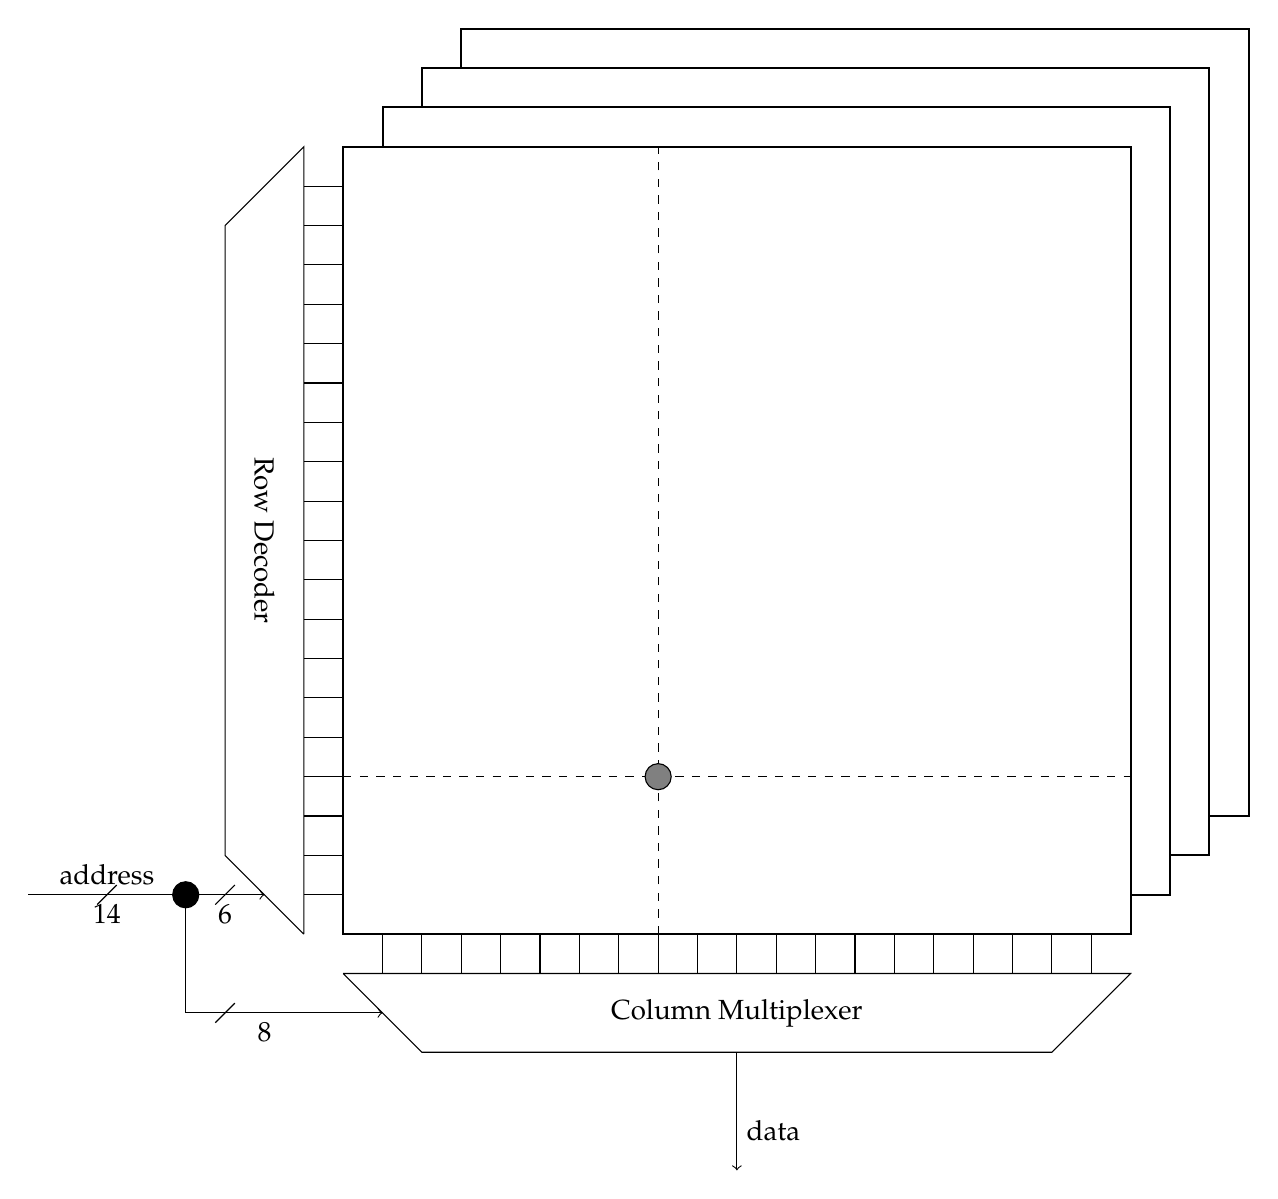
\begin{tikzpicture}
  % matrix square
  \foreach \x in {3,...,0}
    \draw[fill=white, line width=0.25mm] (10 + \x/2, 10 + \x/2) rectangle (20 + \x/2, 20 + \x/2);
  % matrix lines
  \foreach \x in {1,...,19}
    \draw (10 + \x / 2, 9.5)--(10 + \x / 2, 10);
  \foreach \x in {1,...,19}
    \draw (9.5, \x / 2 + 10)--(10, \x / 2 + 10);

  % row decoder
  \draw (9.5, 10)--(9.5, 20)--(8.5, 19)--(8.5, 11)--(9.5, 10);
  \node[rotate=270] at (9, 15){Row Decoder};

  % column multiplexer
  \draw (10, 9.5)--(20, 9.5)--(19, 8.5)--(11, 8.5)--(10, 9.5);
  \node at (15, 9){Column Multiplexer};

  % address lines
  \draw[->] (6, 10.5)--(9, 10.5);
  \draw[->] (8, 9)--(10.5, 9);
  \draw (8, 10.5)--(8, 9);

  % address lines split point
  \node[draw, circle, fill=black] at (8, 10.5){};

  % address lines width markers
  \node[draw, strike out] at (7, 10.5){};
  \node[below] at (7, 10.5){14};
  \node[above] at (7, 10.5){address};

  \node[draw, strike out] at (8.5, 10.5){};
  \node[below] at (8.5, 10.5){6};

  \node[draw, strike out] at (8.5, 9){};
  \node[below] at (9, 9){8};

  % input/output line
  \draw[->] (15, 8.5)--(15, 7);
  \node[right] at (15, 7.5){data};

  % example bit
  \draw[dashed] (10, 12)--(20, 12);
  \draw[dashed] (14, 10)--(14, 20);

  \node[draw, circle, fill=gray] at (14, 12){};

\end{tikzpicture}
\caption{Simplified DRAM internal circuit}
\end{figure}

\memoryname{} is a DRAM actually made by:
\begin{itemize}
  \item 32 matrices: matrix \emph{n} holds the corresponding \emph{n}-th bit of the word connected to the bus;
  each matrix consists of $64 \times 256$ cells;
  each cell holds one bit;
  for practicity, in the above figure, only 4 matrixes have been drawn;
  \item a row decoder: the row decoder is controlled by the 6 most significant bits of the address, and is used to select one of the $2^{6} = 64$ rows of the matrix;
  \item a column multiplexer: the column multiplexer is controlled by the 8 least significant bits of the address, and is used to select one of the $2^{8} = 256$ columns of the matrix;
\end{itemize}

\memoryname{} is compatible with a real world DRAM, and is even simpler, since current memories have up to 64~bit wide buses and up to 8~K rows and columns.
\\
However, note that the above figure does not exactly represent a real DRAM, since some parts of the circuit, like the sense amplifier, have not been drawn because they are not relevant in our discussion.

\subsection{Input and output}
A memory controller is required to actually read and write a DRAM.
It can reside inside the CPU/cache, on an external chip on the computer main board, or inside the memory itself; its positioning and details have not been taken in account, but we must suppose it exists somewhere.

To control and actually read and write a DRAM, the following control lines are used by the memory controller.

\begin{itemize}
  \item \textbf{\textoverline{ras}}: the \emph{row address strobe} signal enables the row decoder circuit;
  \item \textbf{\textoverline{cas}}: the \emph{column address strobe} signal enables the column multiplexer circuit;
  \item \textbf{r/\textoverline{w}}: the \emph{read/write} signal controls if the cell has to be read or written;
  \item \textbf{address}: the \emph{address} line holds the memory address of the cell;
  \item \textbf{data}: the \emph{data} line holds the data read or written from/to the cell;
\end{itemize}

Reading and writing data in the matrix requires strict timing constraints to allow capacitors, sense amplifier and all the electronics to work properly.
Different timings can be used, as explained in the following section.

\section{DRAM control}

\subsection{Simple access} \label{sec:simple-access}
This timing diagram represents the simplest memory cicle that can be used to read and write data in memory.

\begin{minipage}{\textwidth}
\centering
\begin{minipage}{.45\textwidth}
\begin{figure}[H]
\centering
\begin{tikztimingtable}
{\textoverline{ras}}  & H H L L L      L L L L H H\\
{\textoverline{cas}}  & H H H H L      L L H H H H\\
{r/\textoverline{w}}  & H H H H H      4H 2H\\
{addr}                & U 5D{address}  5U \\
{data}                & U 4U           4D{data} 2U\\
\end{tikztimingtable}
\caption{simple read}
\end{figure}
\end{minipage}
\begin{minipage}{.45\textwidth}
\begin{figure}[H]
\centering
\begin{tikztimingtable}
{\textoverline{ras}}  & H H L L L      L L L L H H\\
{\textoverline{cas}}  & H H H H L      L L H H H H\\
{r/\textoverline{w}}  & H H L L L      L H 4H\\
{addr}                & U 5D{address}  5U \\
{data}                & U 4U           4D{data} 2U\\
\end{tikztimingtable}
\caption{simple write}
\end{figure}
\end{minipage}
\end{minipage}

\subsection{Fast page access} \label{sec:fast-page-access}
When accessing data it is possibile to take advantage of the principle of locality.

Usually programs are sequential and have small loops, thus they use to access a small region of memory for a while. Moreover, they usually make computations over the same data for a while.

To take advantage of both the spatial and the temporal locality of programs, it is possible to drive the memory matrix in such a way there is no need to make a complete full simple memory cycle for every access, but some operations can be avoided to save time.

More in details, it is not necessary to deassert the \emph{row address strobe} when memory locations are accessed sequentially and row number does not change.

Proper timing diagrams for fast page access are as the following.
\\
\\
\begin{minipage}{\linewidth}
\centering
\begin{minipage}{.45\textwidth}
\begin{figure}[H]
\centering
\begin{tikztimingtable}
{\textoverline{ras}}  & H H L L L      L L L L L L    L L L L L 3L 2H \\
{\textoverline{cas}}  & H H H H L      L L H H H H    H L L L H 5H\\
{r/\textoverline{w}}  & H H H H H      4H 2H          5H 5H\\
{addr}                & U 5D{address}  4U             4D{address}    7U \\
{data}                & U 4U           4D{data} 2U    U U U 4D{data} 3U\\
\end{tikztimingtable}
\caption{fast page read}
\end{figure}
\end{minipage}
\begin{minipage}{.45\textwidth}
\begin{figure}[H]
\centering
\begin{tikztimingtable}
{\textoverline{ras}}  & H H L L L      L L L L L L    L L L L L 3L 2H \\
{\textoverline{cas}}  & H H H H L      L L H H H H    H L L L H 5H\\
{r/\textoverline{w}}  & H H H H L      2L 2H 2H       2H 3L 5H\\
{addr}                & U 5D{address}  4U             4D{address}    7U \\
{data}                & U 4U           4D{data} 2U    U U U 4D{data} 3U\\
\end{tikztimingtable}
\caption{fast page write}
\end{figure}
\end{minipage}
\end{minipage}
\\
\\
\\
Please note that the first valid address transmitted needs more time to stabilize because it contains both a new row and column address, while subsequent ones need only the time to stabilize the least significant part which represents the column address.

\section{Delay definition}
Analizing previous timing diagrams, these intervals can be observed:
\begin{itemize}
  \item $t_{CL}$ (CAS latency) is defined as the interval between the moment memory controller asserts the \emph{\textoverline{cas}} command and the moment when data is available on memory's output pins;
  \item $t_{RCD}$ (RAS to CAS Delay time) is defined as the delay interval between the CAS assertion and the RAS one;
  \item $t_{RP}$ (RAS Precharge time) is defined as the delay between the RAS assertion and the next command;
  \item $t_{RAS}$ (Active to Precharge Delay) is defined as the delay between the row assertion and the following precharge command;
\end{itemize}

\section{Refresh}
Dynamic RAM cells are made by small capacitors that may hold some electric charge.
Depending on the electric charge held by a capacitor, it can represent an high or a low bit.
Unfortunately, capacitors slowly leak their charge, and need to be refreshed periodically to avoid losing the data stored.
During the refreshing phase, memory can not be accessed.

Time to refresh an entire DRAM can be computed as follow:

$$ t_{R} = r \times t_{RAS} $$

where:

\begin{itemize}
  \item $t_{R}$ is the refresh duration;
  \item $r$ is the number of rows in the memory matrix;
\end{itemize}

To avoid losing too much charge in the capacitors, it is mandatory to refresh all the rows at maximum every 64~ms.
\memoryname{} is implemented with a refresh every 32~ms.

Duration of the interval between two refresh, in terms of number of bus clock cycles, can be computed using the following trivial formula:

$$ n = t_{interval} \times f $$

where:

\begin{itemize}
  \item $ n $ is the number of clock cycles;
  \item $ t_{interval} $ is the duration of refresh interval;
  \item $ f $ is the bus frequency;
\end{itemize}

Thus \memoryname{} is refreshed every $ 32 \times 10^{-3} s \cdot 32 \times 10^{3} Hz = 1024 $ clock cycles.

\section{Interesting cases}
The time needed by the previously described access modes can be computed differently depending on the word that is being accessed and the access mode.
This time mainly depends on the address of the last word accessed, that can lay on the same row or in a different one.

\begin{table}[H]
\centering
\bgroup
\def\arraystretch{1.5}  % add some padding
\begin{tabular}{| c | c | c | c |}\hline
                & first access & same row & different row \\ \hline
  simple access & $t_{RCD} + t_{CL} $ & $t_{RCD} + t_{CL}$ & $t_{RCD} + t_{CL}$\\ \hline
  fast access & $t_{RCD} + t_{CL}$ & $t_{CL}$ & $t_{RP} + t_{RCD} + t_{CL}$ \\ \hline
\end{tabular}
\egroup
\caption{interesting cases delays}
\end{table}
% accessing a bit from a DRAM with the right row open (CL)
% accessing a bit from a DRAM without an active row (t_RCD + t_CL)
% accessing a bit from a DRAM with the wrong row open (t_RP + t_RCD + t_CL)

\section{Simulation}
The described memory has been implemented in an event-driven simulator.

The simulator is organized in modules that interact each other by means of messages. The sending function is scheduled through an event list. Thus when an event occurs, the message associated to such event is forwarded to all modules of the system. The modules are triggered through the \texttt{onNotify} method, inherited from the basic module. Once a module has checked whether it is the message destination, it behaves accordingly to its specifications.

\subsection{Memory module}
In the simplest computer, no cache is present, so memory is directly linked to CPU and must answer only to its requests.
In order to test the \texttt{Memory} module, an additional \texttt{CPUTest} module has been implemented too.
The \texttt{Memory} module is described in the following snippet of code:

\begin{figure}[H]
\lstinputlisting[style=castyle, firstline=35, lastline=65]{../src/memory/memory.h}
\caption{Memory module declaration}
\label{src:memory-h}
\end{figure}

\subsubsection{Member variables}
The \texttt{Memory} module is implemented through the following member variables:

\begin{itemize}
    \item \texttt{dram}: 64KiB \texttt{uint32\_t} array which represents the whole memory;
    \item \texttt{first\_access} and \texttt{last\_row\_addressed}: parameters useful for computing the memory access time;
    \item \texttt{refreshing\_phase} and \texttt{refreshing\_phase\_started\_at}: parameters useful for managing the refresh phase;
    \item \texttt{bus} and \texttt{bus\_status}: variables for interacting with the main bus.
\end{itemize}

\subsubsection{Methods}
\texttt{Memory} operations are defined by the following methods:

\begin{itemize}
    \item \texttt{onNotify(message*)}: inherited from the basic module, it corresponds to the module main program;
    \item \texttt{createMessage(string, string)}: creates a new message according to source and destination parameters;
    \item \texttt{isSelfMessage(message*)}: returns \texttt{true} if the message source is the module itself, \texttt{false} otherwise;
    \item \texttt{onReadRequest(uint16\_t, uint16\_t, string)}: performs the read operation;
    \item \texttt{onWriteRequest(uint16\_t)}: performs the write operation;
    \item \texttt{defaultBehavior()}: computes memory access time without considering the past access history; all accesses take the same amount of time, as described in Section~\ref{sec:simple-access};
    \item \texttt{optimizedBehavior(uint16\_t)}: computes memory access time according to the past access history, as described in Section~\ref{sec:fast-page-access};
    \item \texttt{startRefresh()}: starts the refreshing phase;
    \item \texttt{endRefresh()}: ends the refreshing phase;
\end{itemize}

\texttt{Memory} behavior is depicted in the flowchart diagram in Figure~\ref{fig:flowchart}.

\begin{figure}
    \centering
    \resizebox{0.8\textwidth}{!}{
        % Define block styles
        \tikzstyle{decision} = [diamond, draw, text width=5em, text badly centered, node distance=3cm, inner sep=0pt]
        \tikzstyle{block} = [rectangle, draw, text width=8em, text centered, rounded corners, minimum height=4em]
        \tikzstyle{line} = [draw]

        \begin{tikzpicture}[node distance = 4cm, auto]
            % Place nodes
            \node [block] (init) {initialize module};
            \node [decision, below of=init,  node distance = 4.5cm] (destination) {is destinated to me?};
            \node [decision, below of=destination, node distance = 4.5cm] (selfmessage) {is self message?};
            \node [decision, right of=selfmessage, node distance = 4.5cm] (refresh1) {is refreshing?};
            \node [block, right of=refresh1, node distance = 4.5cm] (endrefresh) {End refresh};
            \node [block, below of=refresh1] (startrefresh) {Start refresh};
            \node [decision, below of=selfmessage, node distance = 4.5cm] (refresh2) {is refreshing?};
            \node [block, left of=refresh2, node distance = 4.5cm] (postpone) {Postpone the request};
            \node [block, below of=refresh2, node distance = 3cm] (bus) {Get the current bus status};
            \node [decision, below of=bus] (read) {is a read request?};
            \node [block, left of=read, node distance = 4.5cm] (update) {Update memory};
            \node [block, right of=read, node distance = 4.5cm] (send) {Prepare the bus and send response};
            \node [block, below of=read] (last) {Update last row used and there will not be first access anymore};
            % Draw edges
            \path [line] (init) -- node {msg received} (destination);
            \path [line] (destination) -- node {yes} (selfmessage);
            \path [line] (selfmessage) -- node {yes} (refresh1);
            \path [line] (refresh1) -- node {yes} (endrefresh);
            \path [line] (refresh1) -- node {no} (startrefresh);
            \path [line] (selfmessage) -- node {no} (refresh2);
            \path [line] (refresh2) -- node {yes} (postpone);
            \path [line] (refresh2) -- node {no} (bus);
            \path [line] (bus) -- (read);
            \path [line] (read) -- node {no} (update);
            \path [line] (read) -- node {yes} (send);
            \path [line] (update) |- (last);
            \path [line] (send) |- (last);
        \end{tikzpicture}
        }
    \caption{Memory simulation flowchart}
    \label{fig:flowchart}
\end{figure}

\subsection{Simulator parameters}
Simulation flow can be altered by means of the following parameters passed as arguments on the command line.

\begin{verbatim}
  $ sim ACCESS_TYPE MODE_TYPE RANDOM_ACCESS_PROB READ_REQ_PROB PRNG_SEED
\end{verbatim}

where

\begin{itemize}
  %\item \texttt{N\_OPERATIONS}: defines number of operations that will be performed;
  \item \texttt{ACCESS\_TYPE}: defines how the access sequence generated; access sequence is a sequence of (address, operation) tuples; it must be chosen among the following two options:
  \begin{itemize}
    \item \texttt{R}: sequence is \emph{real} and is extracted using \emph{pinatrace} tool on a real world test program, provided by Andrea~Mattia Garavagno from the \emph{tracing} team;
    \item \texttt{S}: a \emph{stochastic} sequence is generated randomly using \texttt{*\_PROB} parameters;
  \end{itemize}
  \item \texttt{MODE\_TYPE}: defines page access type; it must be chosen among the following two options:
\begin{itemize}
  \item \texttt{D}: access is performed using the simple \emph{default} access mode, as described in Section~\ref{sec:simple-access};
  \item \texttt{F}: access is performed using the fast page access \emph{fast} mode, as described in Section~\ref{sec:fast-page-access};
\end{itemize}
  \item \texttt{RANDOM\_ACCESS\_PROB}: defines the probability of a random access, where \texttt{100} means totally random access and \texttt{0} means totally sequential access;
  \item \texttt{READ\_REQ\_PROB}: defines the probability that an access is a read or a write, where \texttt{100} means that every access will be a read, while \texttt{0} means that every access will be a write;
  \item \texttt{PRNG\_SEED}: defines the seed of the pseudo-random numbers generator; the Mersenne Twister pseudo-random generator provided by C++ STL has been used;
\end{itemize}

\section{Test}
% 5 tests have been done with different seeds for the random number generator, and average of results has been calculated, in order to avoid possible biases due to a certain pseudorandom sequence

% which tests did we do?
% Gerry knows

\section{Transfer speed}
Since this is a \emph{single data rate} memory, in short SDR, it is theoretically possible to read or write data from/to the memory once for every rising edge of the bus clock.

Thus, maximum theoretical transfer speed is given by the following formula:

$$ s_{max} =  f \cdot B_w $$

where

\bgroup
\def\arraystretch{1.5}
\begin{table}[H]
\center
\begin{tabular}{| c | c | c |}\hline
\textbf{symbol} & \textbf{unit} & \textbf{description} \\ \hline
$ s_{max} $ & $ \frac{bit}{s} $ & maximum theoretical speed \\ \hline
$ f $ & Hz & bus frequency \\ \hline
$ B_{w} $ & bit & bus width \\ \hline
\end{tabular}
\end{table}
\egroup

Thus, \memoryname{} has a maximum theoretical transfer speed of $32 \times 10^{3} Hz \cdot 32 = 1.024 Mbit/s = 128 KiB/s $.

\section{Conclusion}
% as we have seen using our test «benchmarks» the two different access modes for sequential read/write the fast page mode access is better
% «strategic»
% «negligible»

\end{document}
